%!TEX root=/home/ska124/Dropbox/Thesis/thes-full.tex

%%%%%%%%%%%%%%%%%%%%%%%%%%%%%%%%%%%%%%%%%%%%%%%%%
%
%     Chapter 4   
%
%%%%%%%%%%%%%%%%%%%%%%%%%%%%%%%%%%%%%%%%%%%%%%%%

\chapter{Triangulation}
\label{chap:triangulation}

\section{What is Triangulation?}
\label{sec:triangulation}
\alert{Give an example here of each step}



\section{Related Work}
 Consider a source language \emph{s}, pivot language \emph{p} and target language \emph{t}. When using the \emph{cascading} approach, we build two systems, between \emph{s} and \emph{p} and between \emph{p} and \emph{t}. Given a test set in \emph{s}, it is first translated to \emph{p} and those output translations are then translated into the target language \emph{t}, making decoding twice as expensive as well. We do not report our results on using cascading for various reasons. Firstly, translating the output of a source pivot system trained and tuned on little data will lead to propogation of errors. Secondly, we will need three development sets, one for each system. Finding standard development sets for low-resource languages is unlikely. Finally, it has been shown before that cascading does not give the most fluent translations.~\newcite{Utiyama:07} compared pivot-based triangulation with cascading using all of multi-parallel europarl, observing that pivot-based methods outperformed cascading.

 The second approach is the pivot-based approach where a triangulated phrase table is generated between the source and target, by using the common pivot phrases between the source pivot and pivot target tables~\cite{Utiyama:07,Cohn:07}.~\newcite{Utiyama:07} observed that the triangulated table was able to achieve comparable BLEU scores to the direct system for French, German and Spanish. This could be owing to the fact that the data comprised multi-parallel 560K sentences.~\newcite{Cohn:07} observe that multiple pivot languages lead to more fluent translations compared to one pivot language. Multiple pivot language lead to multiple alternative translations, thus, increasing phrase coverage and rewarding the more appropriate translations and reducing out-of-vocabulary words further. They also propose a systematic way of combining the triangulated translation model with the direct model using linear interpolation and log-linear interpolation, although they assume a uniform weight for both the models. To ``simulate'' a low-resource scenario, the top 10K multi-parallel sentences are considered for source pivot, pivot target and source target systems. As we will observe later, real low-resource scenarios are significantly different from how it was simulated in~\cite{Cohn:07}.~\cite{Nakov:12} propose a language-independent approach to improving translation for low-resource languages, but the approach assumes the presence of a resource-rich language that bears similarity to the low-resource language, the similarities helping in creating a large triangulated phrase table. In~\cite{Nakovemnlp:12}, the resource-rich language is adapted to be more like the resource-poor one. Notice that this also assumes both are very similar. Results are reported using both Malay-Indonesian and Bulgarian-Macedonian, the third language being English in both cases.~\cite{Gispert:06} translate Catalan to Spanish via English by using news corpora on both source pivot and pivot target side.~\cite{Huck:12} report on BLEU score improvements by using $10^9$ parallel sentence between German and French.

 
 A common thread that binds the previous work using the approach of Triangulation is the usage of resource-rich languages. The fundamental reason behind the effectiveness of Triangulation is the reduction in the number of OOVs when using the pivot language(s). This can be observed in various forms. If the source and pivot language have a healthy vocabulary overlap, the SMT system between source-pivot is large, thus, improving translations. This factor also helps when the amount of parallel text between source-pivot is relatively low, e.g, Indonesian-English.  All the europarl languages are based on parlimentary proceedings and have minimal noise. Hence, the improvements using triangulation over the direct systems cannot be generalized for systems for low-resource languages. All the papers that use triangulation in machine translation cite either \cite{Utiyama:07} or \cite{Cohn:07}, both published in 2007 (and sometimes cite both of them but use either one model or the other). However, these two papers introduce triangulation for phrase-based SMT in very different ways and their models are different from each other. To our knowledge, before this dissertation, there has been no in-depth study of the different choices in building an SMT system using triangulation. Another limitation of the original work in triangulation~\cite{Utiyama:07,Cohn:07} is the unrealistic use of languages with abundant parallel data to simulate low-resource languages. Subsequent work~\cite{Nakov:12,Nakovemnlp:12,Gispert:06,Huck:12} has also assumed that parallel data in pivot languages can be found in the same domain as the original resource-poor language pair. This kind of domain similarity is not easy to find for realistic low-resource settings.

 ``Simulating'' low-resource scenarios is ineffective in various ways. Firstly, real low-resource languages are noisy, not perfectly sentence aligned, and do not have a lot of data in the target domain. Secondly, triangulation is highly dependent on how good is the source pivot bitext. If the size of source pivot bitext is comparable to the source target, and/or is in the same domain, this increases bias in triangulation by introducting several common phrases, and, this is also not seen in a real low-resource setting.


 Consider a source language, \emph{s}, a target language, \emph{t}, and a pivot language \emph{p}. You have a little parallel data between \emph{s} and \emph{t} and believe that triangulation will increase the quality of translations between \emph{s} and \emph{t}. What steps one would follow to get the desired result ?

\begin{algorithm}
\caption{Triangulate}
\textbf{Input:} phrase table between \emph{s} and \emph{p}, p$_{src-pivot}$, \\
 phrase table between \emph{p} and \emph{t}, p$_{pivot-tgt}$,  \\
 \emph{n} for selecting top-n phrase pairs \\
\textbf{Output:} p$_{trian}$
\begin{algorithmic}
\FORALL{(src, pivot) in top-\emph{n} p$_{src-pivot}$} \IF{pivot phrase in p$_{pivot-tgt}$}

        \FOR{all (pivot, tgt) pairs in p$_{pivot-tgt}$}
        \STATE{find scores for p$_{src-tgt}$}
        \ENDFOR
        \STATE{select top-\emph{n} src-target pair, add to p$_{trian}$}
        \ENDIF
        \ENDFOR


%\ENDFOR
\end{algorithmic}

\end{algorithm}

\begin{equation}
 p_{lex}(t \mid s) = \Sigma p_{lex}(t \mid i) p_{lex}(i \mid s)
\end{equation}

\begin{equation}
	p_{lex}(s \mid t) = \Sigma p_{lex}(s \mid i) p_{lex}(i \mid t)
\end{equation}

\begin{equation}
	p_w(t \mid s) = \Sigma p_w(t \mid i) p_w(i \mid s)
\end{equation}

\begin{equation}
	p_w(s \mid t) = \Sigma p_w(s \mid i) p_w(i \mid t)
\end{equation}

In~\cite{Cohn:07}, 

\begin{eqnarray*}
p(t \mid s)&=&\sum_{i}{p(t, i \mid s)}\\
&=& \sum_{i}{p(t \mid i, s)\,p(i \mid s)}\\
&\approx& \sum_{i}{p(t \mid i)\,p(i \mid s)}
\end{eqnarray*}

\section{Translation Model Combination}
\label{sec:interpolation}

	Combining translation models, trained on corpora from different domains, is an inherently difficult task. We want to make our translations better on the domain of the test set, while also correcting errors in our baseline translation model. In case of low-resource languages, the baseline translation model has been trained on completely out-of-domain corpora or some in-domain and a lot of out-of-domain corpora. This results in translation pairs that are missing altogether or translation pairs with so low probability that decoding misses them altogether. The aim of Interpolation is to add translation pairs that are missing and give more weightage to translations that are more valid in the given domain. 

	Consider the translations from Haitian-Creole to English. We have a baseline model trained on a little in-domain parallel data (\~17K sentences). We aim to make our translations better on the same domain using a lot of out-of-domain data, which in our case is parlimentary proceedings. Its important that we do not make the baseline model translations end up at the bottom of the stack because they are in-domain. At the same time, we do not want to miss out on the valid translations introduced by the larger, clean parliamentary proceedings based translation model. 

	\subsection{Example}
		Consider a phrase pair, (jan nou, that you). Each phrase pair has a set of scores associated with it in the phrase table. They are the forward and backward lexical probabilities, and the forward and backward phrase probabilities. 

		From the direct phrase table, we have the following scores for the phrase pair mentioned above. The last score, 2.718, is a constant which is the phrase penalty. 
	\begin{verbatim}
		jan nou  ||| that you ||| 0.000786782 2.11603e-05 0.125 0.00906772 2.718 
	\end{verbatim}

		The triangulated table also happens to have the same phrase pair with different scores. These scores have been obtained by using the equations shown above.
	\begin{verbatim}
		jan nou ||| that you ||| 0.00318015 7.75194e-05 0.0715829 0.00214831 2.718
	\end{verbatim}

		We know that our direct system has been trained on in-domain data, hence, it should get more weightage intuitively. A heuristic approach to this problem would choose a pair of values and see which one does best. For instance, if you choose 0.85 for the direct table and 0.15 for the triangulated table, the end result for the phrase pair would look like the following : 

	\begin{verbatim}
		jan nou ||| that you ||| 0.0011457872 2.961416503e-05 0.116987435 0.00802980849 2.718	
	\end{verbatim}

		There are several flaws with the approach outlined above. Firstly, an intuitive idea about the importance of the in-domain or out-of-domain phrase table is not enough. The direct Haitian-creole to English phrase table has been trained on only 110K parallel sentences and cannot always be right. Hence, starting with 0.9 for the direct table and 0.1 for the triangulated table is an extreme step. So is 0.5 and 0.5 because we want translations with more influence from the cleaner, larger Europarl data. Moreover, as we will discuss in the other chapters, we report results on several combinations of triangulation, based on changes in phrase scores, lexical scores and adding connectivity features. With every improvement, the importance of the triangulated table might increase or decrease. The heuristic approach will not be able to take that into account. 

		We use CONDOR to perform an efficient grid search over the pairs of co-efficients based on the BLEU score of the interpolated system on the heldout set. Our intepolation method would have the following steps : 
 
		\begin{itemize}
			\item Start with a number, say, 0.85 and 0.15
			\item Interpolate baseline and triangulated. Run MERT with the interpolated table
			\item Get the BLEU of this set of weights on heldout set
			\item Based on the BLEU score, Condor generates a new pair of co-efficients
		\end{itemize}



\section{Europarl}
Europarl refers to the parallel corpora generated by translating the proceedings of European parliament into several languages. Version 7 of Europarl now has 20 languages, from French to Estonian and Finnish. Release of the Europarl corpus led to a surge in research into more and more data-driven methods to enable Statistical Machine Translation. The results were easily reproducible and the data is very clean and sentence-aligned. 

Moreover, Europarl is multi-parallel. What does multi-parallel imply? Consider english as the common target language. A multi-parallel corpora between 20 European languages and English comprises sentences in 20 european languages which translate to the same english sentence. 

\begin{figure}[ht]
	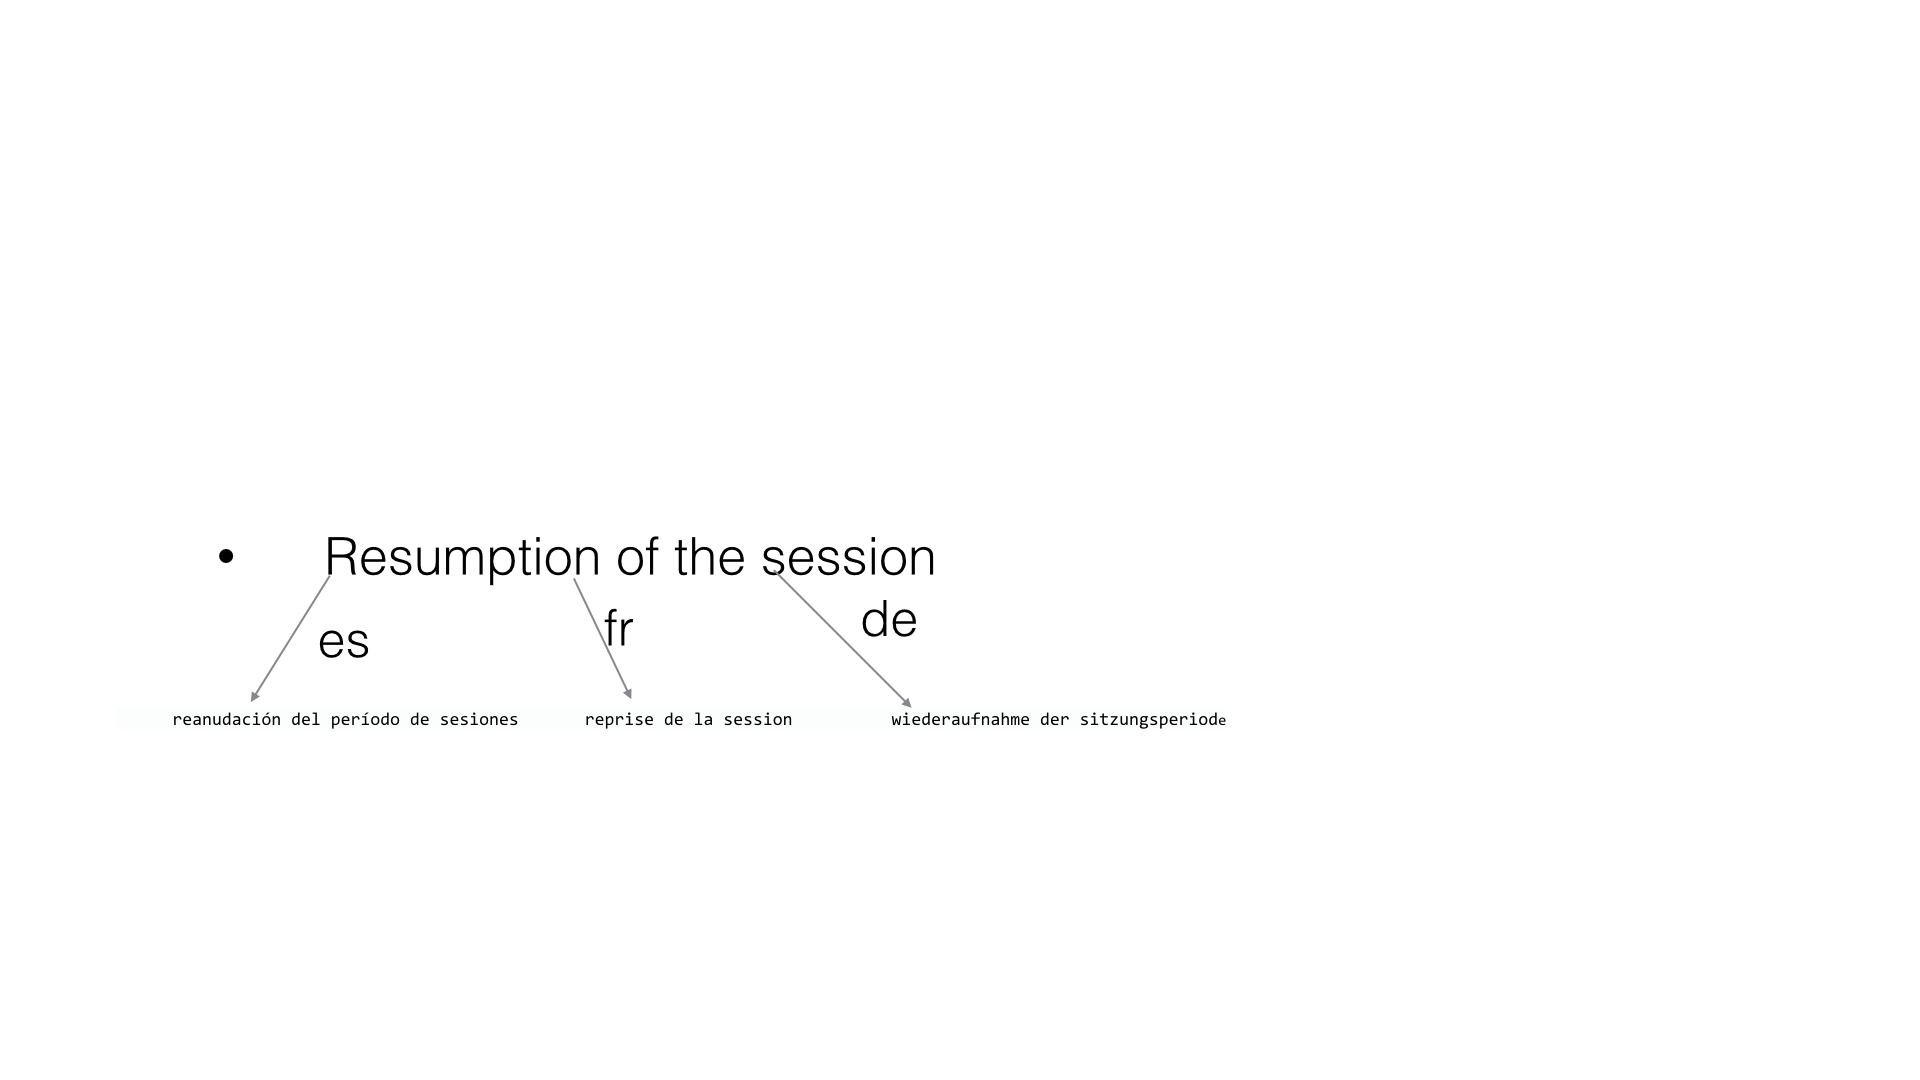
\includegraphics[trim=4cm 4cm 4cm 4cm, height=0.5\textheight, clip=true]{files/Figures/eparl_multiparallel.jpg}
	\caption{Spanish = es, French = fr, German = de}
	\label{fig:eparl_multi}
	\small
	\centering
\end{figure}



\section{Low-resource simulation}

\cite{Cohn:07} simulated ``low-resource'' settings by using the top 10K sentences for the source pivot, pivot target and source target systems.  

\begin{figure}[ht]
	\small
	\centering
	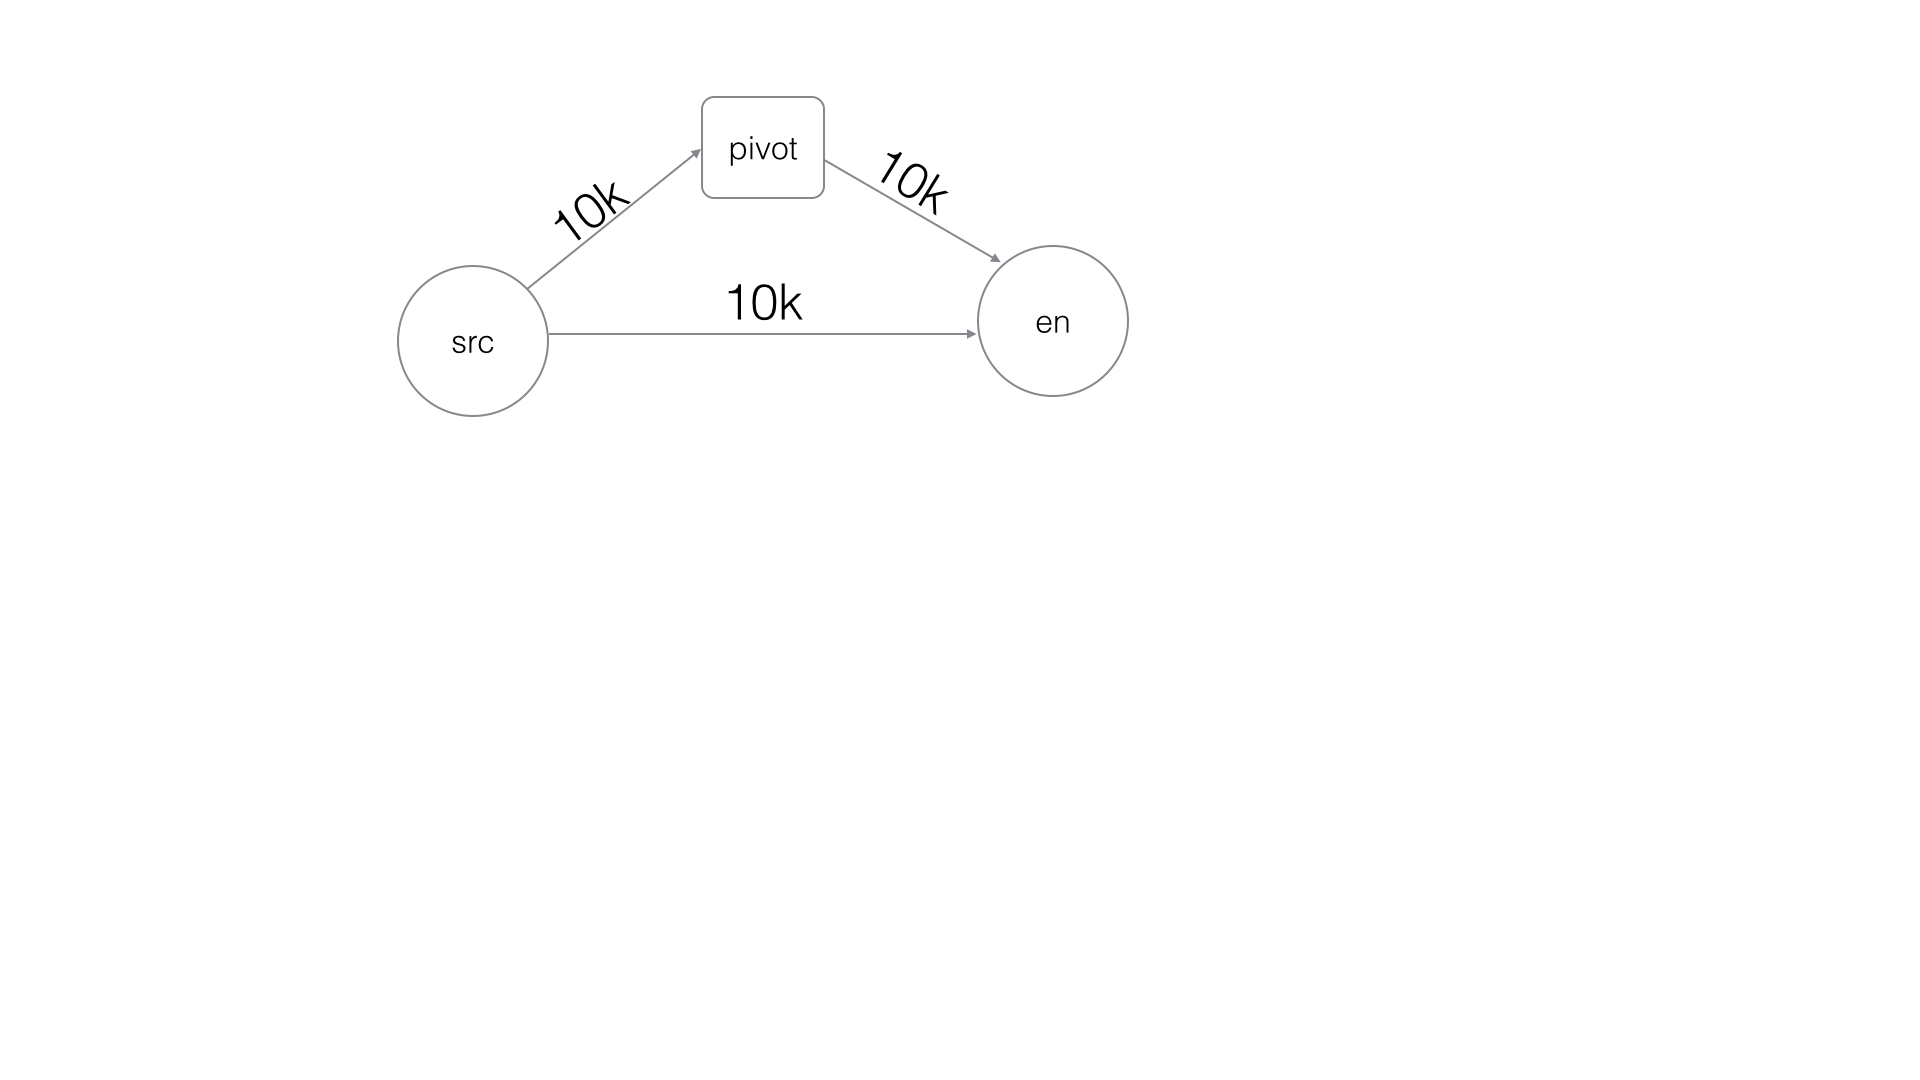
\includegraphics[trim=2cm 4cm 4cm 4cm, height=0.6\textheight]{files/Figures/Cohn.jpg} 
	\caption{Low-resource simulation in Cohn \& Lapata, '07}
	\label{fig:Cohn_lowresource}
\end{figure}

\begin{figure}
	\small
	\centering
	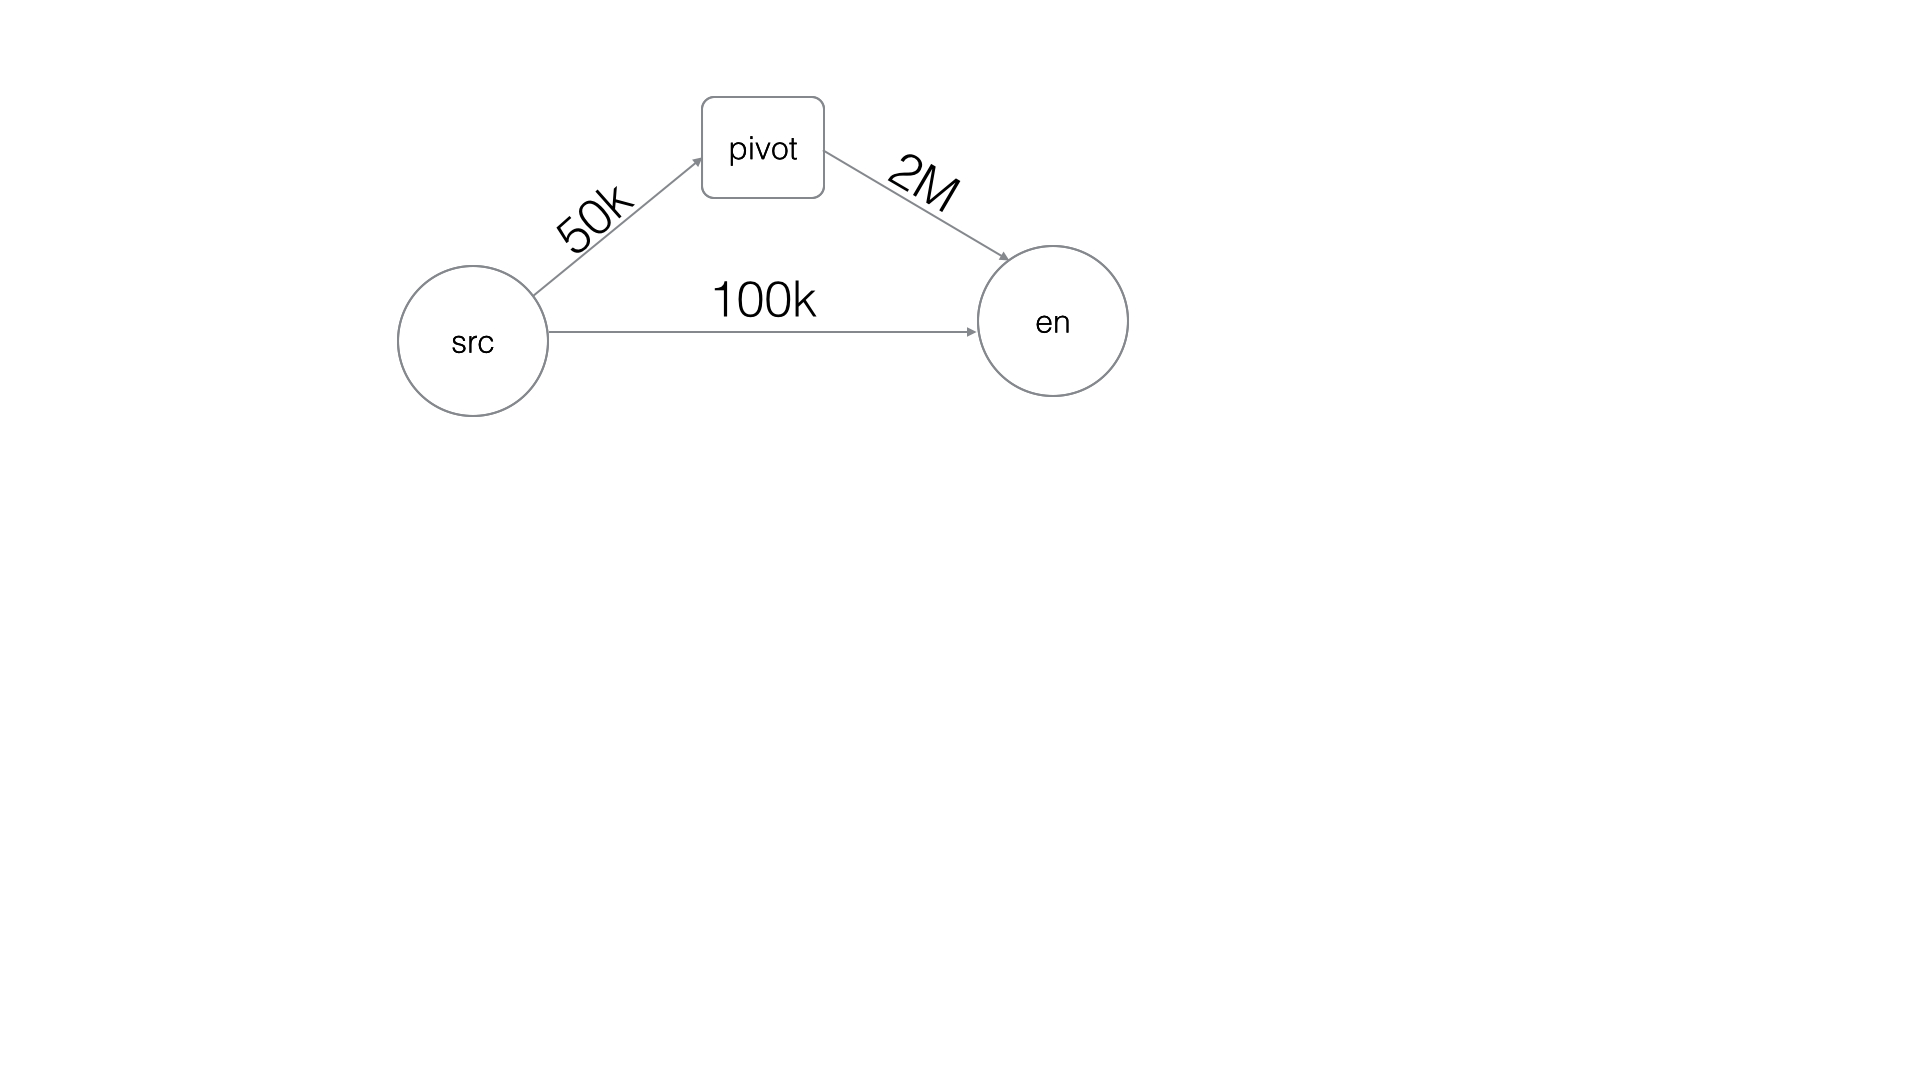
\includegraphics[trim=2cm 4cm 4cm 4cm, height=0.5\textheight]{files/Figures/Our.jpg} 
	\caption{Our low-resource simulation setting}
	\label{fig:our_setting}
\end{figure}



\section{Experiments}
\begin{figure}[ht]
	\small
	\centering

	\begin{tabular}{lr}

\toprule
System & BLEU \\
\toprule
es-en & 23.32 \\
fr-en & 19.53 \\
de-en & 15.60 \\
\bottomrule
\centering
\small
\label{table:eparl100}
\end{tabular}
	\label{table:eparlbaselines}
	\caption{Europarl Baselines - 100K}
\end{figure}

 \begin{figure}[ht]
 	\small
 	\centering
	\begin{tabular}{lrrrrrr}
\toprule

src-tgt & pivot & top20 & top40 & top60 & top80 & top100 \\
\toprule

de-en & fr & 13.32 & 13.33 & 13.35 & 13.42 & 13.03 \\
de-en & es & 13.37 & 13.17 & 13.49 & 13.34 & 13.36 \\
fr-en & de & 16.21 & 15.82 & 15.89 & 16.08 & - \\
fr-en & es & 17.77 & 18.15 & 17.99 & 18.01 & 18.27 \\
es-en & fr & 21.35 & 21.18 & 20.83 & 21.01 & 21.45\\
es-en & de & 18.36 & 19.19 & 19.35 & 19.23 & 18.97 \\
\bottomrule
\centering 
\small
\label{table:eparltopn}
\end{tabular}
 
	\label{table:eparltopn}
	\caption{BLEU scores when just using the triangulated table}
 \end{figure}


\section{Translation Model Combination}

\begin{figure}[ht]
	\small
	\centering
	\begin{tabular}{llrrrrrr}
\toprule
src-tgt & pivot & baseline & top20 & strength & M1 & joint & all \\
\toprule
de-en & fr & 15.60 & 15.45 & - & 15.24 & - & -  \\
de-en & es & 15.60 & 15.55 & - & 15.49 & - & - \\
fr-en & de & 19.53 & 19.85 & - & 19.92 & - & - \\
fr-en & es & 19.53 & 19.86 & - & 20.03 & - & - \\
es-en & fr & 23.32 & 23.66 & - & 23.85 & - & - \\
es-en & de & 23.32 & 23.68 & - & 23.84 & - & - \\
\bottomrule
\centering
\small
\label{table:eparlintertopn}
\end{tabular}
	\label{table:eparltopninter}
	\caption{BLEU scores with top-20 interpolation}
\end{figure}




%\section{Using Bible}

%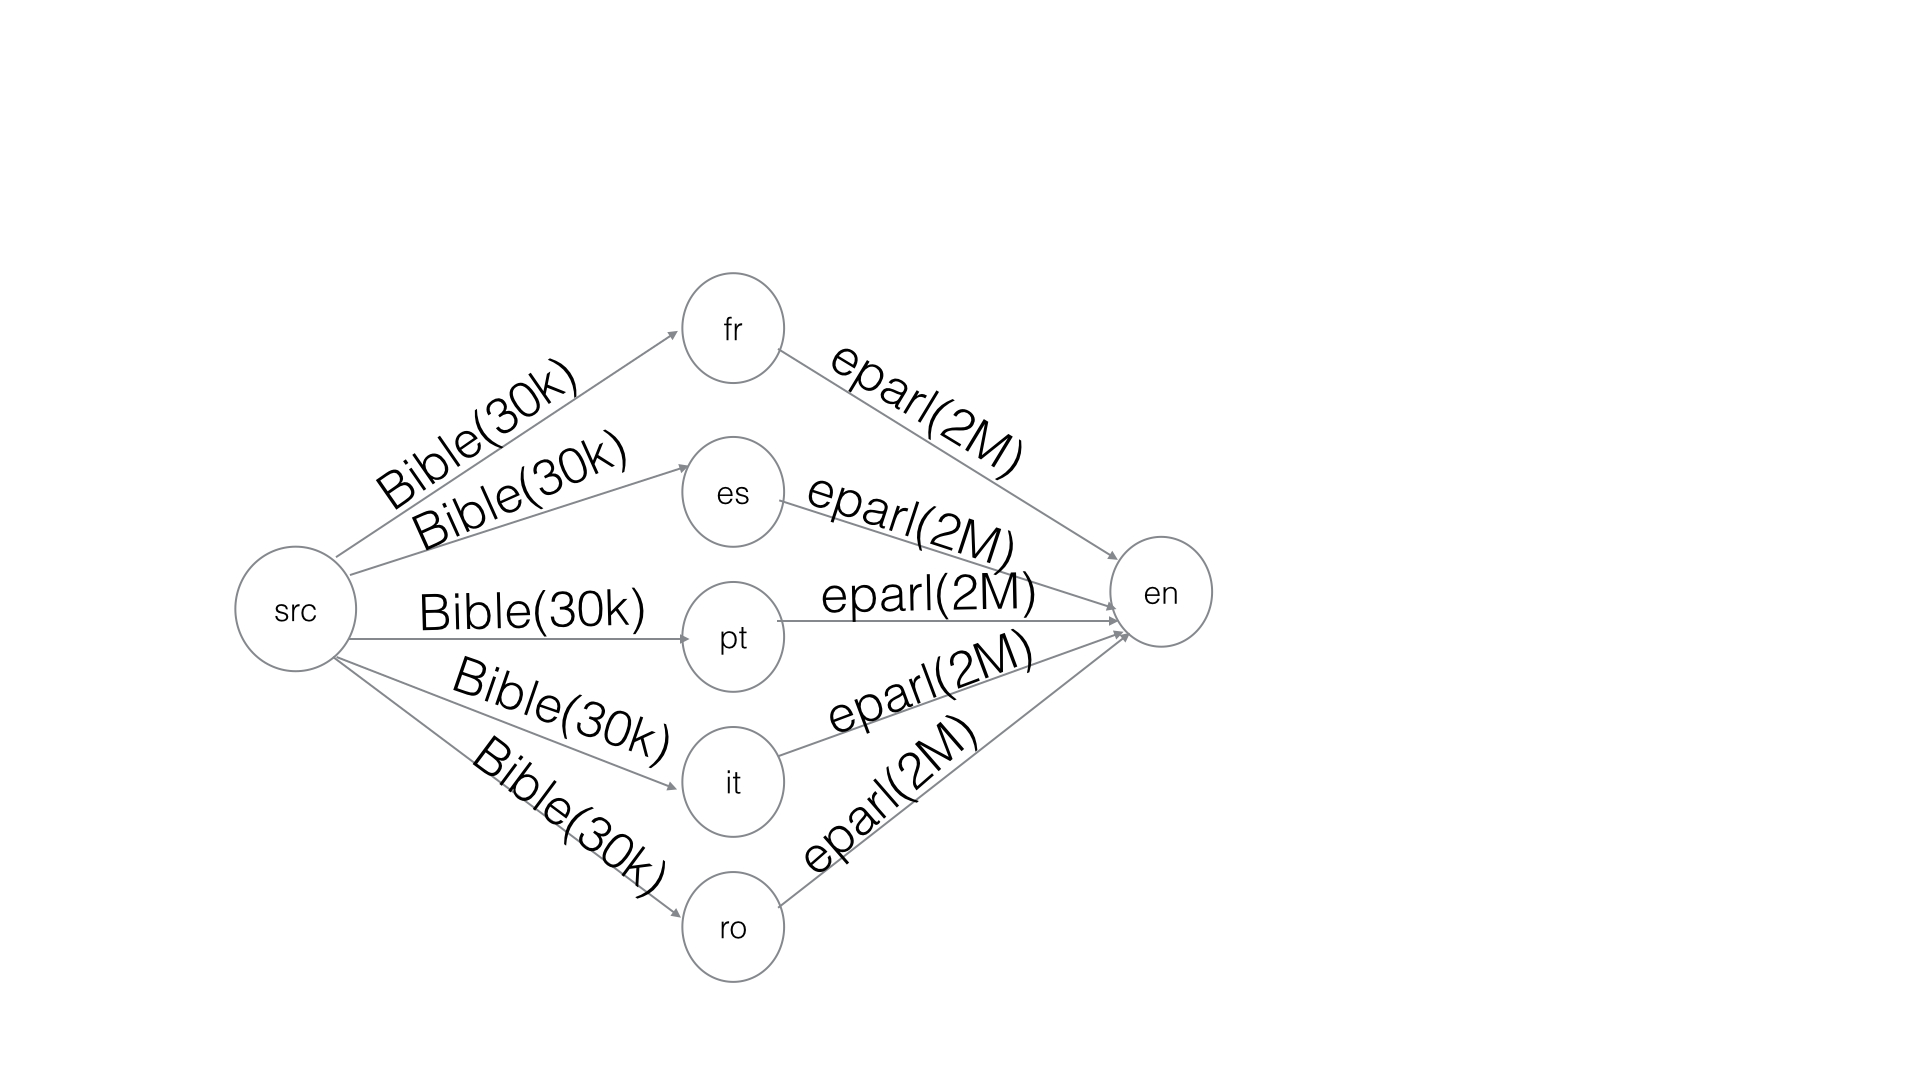
\includegraphics[scale=0.4]{files/Figures/pivot.jpg}





